\documentclass[]{beamer}

\usetheme{Pittsburgh}
\usecolortheme{dove}

\usepackage[]{amsmath}
\usepackage{amssymb}
\usepackage{cmbright}
\usepackage[]{graphicx}
\usepackage{bm}

\newcommand{\RR}{\mathbb{R}}
\newcommand{\abs}[1]{|#1|}
\newcommand{\set}[1]{\{ #1 \}}
\newcommand{\defkey}{\textbf}

\title{Measuring polygonal niceness}
\author[Duppala, Kraemer]{%
Sharmila Duppala\inst{1}, %
David Kraemer\inst{1}}

\institute[Stony Brook University]
{
  \inst{1}%
  AMS 545: Computational Geometry \\
  Stony Brook University
}

\date[2018]{May 1, 2018}


\begin{document}

\frame{\titlepage}

\begin{frame}[t]{Preliminaries}
  \begin{itemize}
    \item $\lambda(A)$ is the area of a set $A \subseteq \RR^2$.
    \item Let $P \subseteq \RR^2$ denote a simple bounded closed polygon.
    \item $\partial P$ is the boundary of $P$.
    \item $\abs{\partial P}$ is the perimeter of $P$.
    \item $[x,y]$ is the closed line segment bounded by $x,y \in \RR^2$.
  \end{itemize}
\end{frame}

\begin{frame}[t]{Measures of niceness}
  \begin{definition}[$\alpha$-fatness]
    The \defkey{$\bm{\alpha}$-fatness score} is given by
    \begin{equation*}
      \alpha(P) = \inf\set{
        \frac{\lambda(B(x, \rho) \cap P)}{\lambda(B(x, \rho))} : \rho > 0
      }
    \end{equation*}
    where $x \in P$, and $B(x,\rho)$ is a ball centered at
    $x$ not containing $P$.
  \end{definition}
  \begin{itemize}
    \item The ``minimizing'' ball might contain $P$.
    \item Find the smallest such proportion. This is $\alpha(P)$.
    \item It's much easier when the ball is a square!
  \end{itemize}
\end{frame}

\begin{frame}[t]{Measures of niceness}
  \begin{itemize}
    \item Let $R$ be a rectangle with length $\ell$ and height $h$. (WLOG, $\ell
      \geq h$.) Then
      \begin{equation*}
        \alpha(R) = \frac{h}{4\ell}.
      \end{equation*}
  \end{itemize}
  \begin{center}
    \includegraphics[width=0.55\textwidth]{../plots/alpha_fatness_rectangle.eps}
  \end{center}
\end{frame}

\begin{frame}[t]{Measures of niceness}
  \begin{itemize}
    \item Let $C$ be a circle with radius $r$. Then 
      \begin{equation*}
        \alpha(C) = \frac{\pi r^2}{16r^2} = \frac{\pi}{16} < \frac{1}{4}.
      \end{equation*}
  \end{itemize}
  \begin{center}
    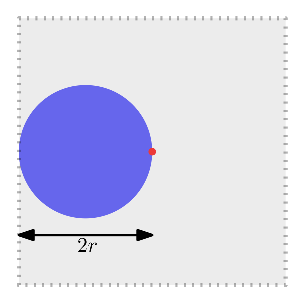
\includegraphics[width=0.55\textwidth]{../plots/alpha_fatness_circle.eps}
  \end{center}
\end{frame}


\begin{frame}[t]{Measures of niceness}
  \begin{definition}[Chord-arc]
    The \defkey{chord-arc score} is given by
    \begin{equation*}
      s_p (P) =
      \inf\set{\max( \abs{\partial P'}, \abs{\partial P''}): x,y \in \partial P},
    \end{equation*}
    where the chord $[x,y]$ partitions $P = P' \cup P''$.
  \end{definition}
  \begin{itemize}
    \item This is a ``minimax'' definition. We want the least bad resulting split.
    \item The polygon perimeter is computed by summing the ``lengths'' of each
      boundary edge.
    \item Here $p$ indicates a norm. Ideally $p = 2$, but for computation
      purposes we choose $p = 1$ or $p= \infty$.
  \end{itemize}
\end{frame}

\begin{frame}[t]{Measures of niceness}
  \begin{itemize}
    \item Let $R$ be a rectangle with length $\ell$ and height $h$. (WLOG, $\ell
      \geq h$.) Then
      \begin{equation*}
        s_p(R) = 2h + \ell
      \end{equation*}
  \end{itemize}
  \begin{center}
    \includegraphics[width=0.65\textwidth]{../plots/chord_arc_rectangle.eps}
  \end{center}
  \begin{itemize}
    \item This holds for many $p$.
  \end{itemize}
\end{frame}

\begin{frame}[t]{Stray observations}
  \begin{itemize}
    \item The $\alpha$ fatness score seems to penalize oblong polygons and
      reward ``squarely compact'' polygons.
    \item The chord-arc score seems to penalize local nonconvexity. 
    \item Remember that we want a large $\alpha$ score but a small chord-arc
      score.
  \end{itemize}
\end{frame}

\begin{frame}[t]{Implementation}
  \begin{itemize}
    \item The measurements were implemented in C++ using CGAL with exact
      arithmetic kernel.
    \item We used a $\delta$-boundary discretizing scheme: the length of $[x_k,
      x_{k+1}]$ is at most $\delta > 0$ for consecutive boundary vertices.
    \item Generating useful test polygons was tricky.
    \item We ran our measurements on
      \begin{itemize}
        \item Special internally generated nice polygons,
        \item Randomly generated ``typical'' polygons (courtesy of Professor
          Mitchell),
        \item (Simplified) US state boundaries.
      \end{itemize}
  \end{itemize}
\end{frame}

\begin{frame}[t]{Randomly generated polygons} 
  \includegraphics[width=\textwidth]{../plots/u_100_alpha_score_chord_arc_infinity_vertices_0-05_delta_ranking.eps}
  ($\delta  = 0.05$)
\end{frame}

\begin{frame}[t]{Randomly generated polygons}
  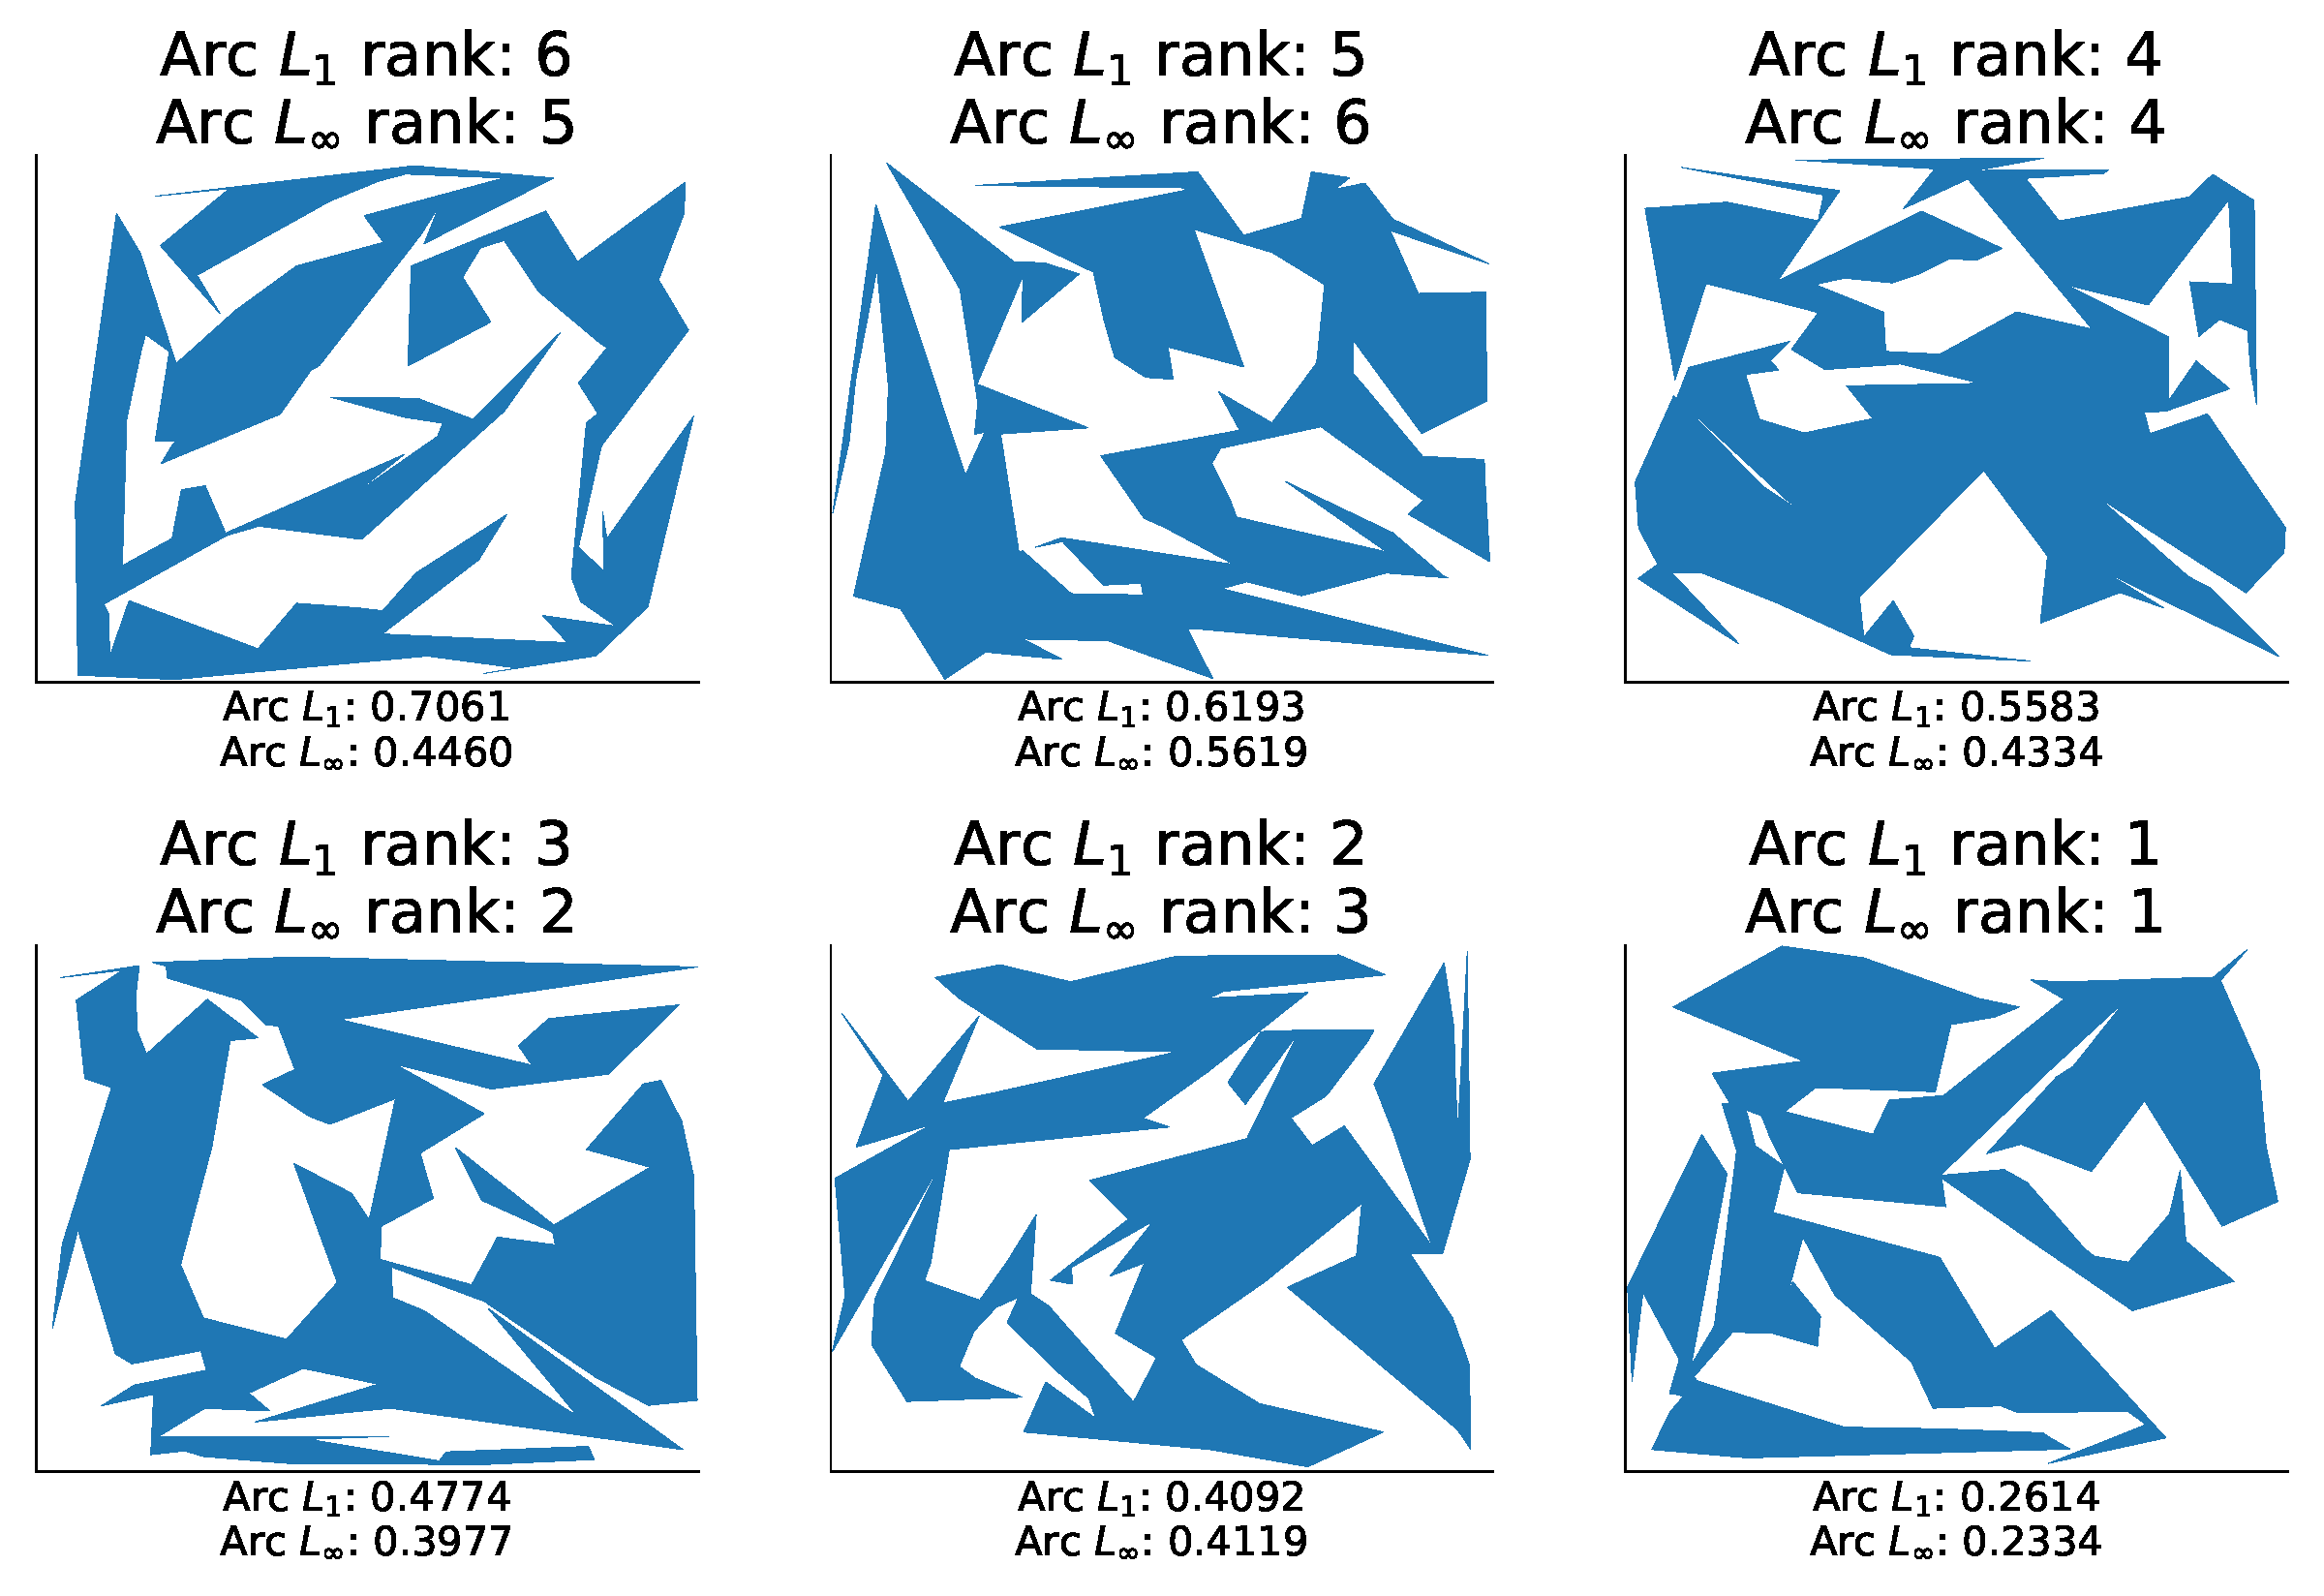
\includegraphics[width=\textwidth]{../plots/u_100_chord_arc_one_chord_arc_infinity_vertices_0-05_delta_ranking.eps}
  ($\delta  = 0.05$)
\end{frame}

\end{document}
